% Gabarit pandoc des corrigés publiés (brut et guidé). Contenu sans marque ni nom de site.
% Compilation : lualatex (latexmk -lualatex).
% Le Markdown reste la source unique : ne pas éditer ce fichier .tex à la main.
\documentclass[11pt,a4paper]{article}

% --- Moteur, polices (Latin Modern) et langue ---------------------------------
\usepackage{iftex}
\ifLuaTeX\else\errmessage{Ce document se compile avec lualatex}\fi
\usepackage{amsmath,amssymb,mathtools}
\usepackage{fontspec}
% mathrm=sym : \mathrm prend ses glyphes dans la police mathématique (ℓ, μ, Ω), comme KaTeX.
\usepackage[math-style=TeX,bold-style=TeX,mathrm=sym]{unicode-math}
% Repli pour les glyphes absents de Latin Modern (indices et exposants Unicode,
% flèches, filets des schémas en texte, symboles) : DejaVu, puis Latin Modern Math
% (ℓ, lettres mathématiques Unicode des légendes).
\directlua{
  luaotfload.add_fallback("repliTexte", {"DejaVuSerif:mode=harf;", "DejaVuSans:mode=harf;", "file:latinmodern-math.otf:mode=harf;"})
  luaotfload.add_fallback("repliMono", {"DejaVuSansMono:mode=harf;", "DejaVuSans:mode=harf;", "file:latinmodern-math.otf:mode=harf;"})
}
\setmainfont{Latin Modern Roman}[RawFeature={fallback=repliTexte}]
\setsansfont{Latin Modern Sans}[RawFeature={fallback=repliTexte}]
\setmonofont{Latin Modern Mono}[RawFeature={fallback=repliMono}]
\setmathfont{Latin Modern Math}
\usepackage[french]{babel}
\frenchsetup{SmallCapsFigTabCaptions=false}

% --- Mise en page --------------------------------------------------------------
\usepackage[a4paper,margin=2.2cm,headheight=14pt,footskip=1.2cm]{geometry}
\usepackage{microtype}
\setlength{\emergencystretch}{4em}
\tolerance=1500
\setlength{\parindent}{0pt}
\setlength{\parskip}{0.55\baselineskip plus 2pt minus 1pt}
\usepackage{xcolor}
% Gris nommés : babel-french rend « ! » actif dans le document.
\definecolor{gris2}{gray}{0.98}
\definecolor{gris3}{gray}{0.97}
\definecolor{gris5}{gray}{0.95}
\definecolor{gris35}{gray}{0.65}
\definecolor{gris40}{gray}{0.60}
\definecolor{gris45}{gray}{0.55}
\definecolor{gris50}{gray}{0.50}
\definecolor{gris55}{gray}{0.45}
\definecolor{gris60}{gray}{0.40}
\definecolor{gris65}{gray}{0.35}
\definecolor{gris70}{gray}{0.30}
\definecolor{gris80}{gray}{0.20}
\definecolor{gris85}{gray}{0.15}
\usepackage{graphicx}
\usepackage{float}
\usepackage{caption}
\captionsetup{font=small,labelformat=empty,justification=centering}
\usepackage{booktabs,longtable,array,multirow,calc}
\usepackage{siunitx}
\sisetup{locale=FR}
\usepackage[version=4]{mhchem}
\usepackage{listings}
\usepackage{fancyhdr}
\usepackage{lastpage}
\usepackage[most]{tcolorbox}
\usepackage{enumitem}
\setlist{nosep,leftmargin=*,topsep=2pt}
\usepackage[hidelinks,unicode]{hyperref}
\usepackage{bookmark}
\hypersetup{pdftitle={CCINP TPC — Mathématiques 2026},pdfauthor={Rédigé par IA},pdfcreator={LaTeX},pdfsubject={Corrigé brut}}
\usepackage{xurl}

% --- Pandoc : listes, tableaux, figures ----------------------------------------
\providecommand{\passthrough}[1]{#1}
\providecommand{\tightlist}{\setlength{\itemsep}{0pt}\setlength{\parskip}{0pt}}

\makeatletter
\def\maxwidth{\ifdim\Gin@nat@width>\linewidth\linewidth\else\Gin@nat@width\fi}
\def\maxheight{\ifdim\Gin@nat@height>0.55\textheight 0.55\textheight\else\Gin@nat@height\fi}
\makeatother
\setkeys{Gin}{width=\maxwidth,height=\maxheight,keepaspectratio}
\setcounter{secnumdepth}{-\maxdimen}
\providecommand{\pandocbounded}[1]{#1}

% --- Code (listings) -----------------------------------------------------------
\lstset{
  basicstyle=\ttfamily\small,
  columns=fullflexible,
  keepspaces=true,
  breaklines=true,
  breakatwhitespace=false,
  postbreak=\mbox{\textcolor{gris50}{$\hookrightarrow$}\space},
  frame=single,
  rulecolor=\color{gris35},
  framesep=4pt,
  xleftmargin=5pt,xrightmargin=5pt,
  backgroundcolor=\color{gris3},
  keywordstyle=\bfseries,
  commentstyle=\color{gris65},
  stringstyle=\color{gris80},
  showstringspaces=false,
  tabsize=4,
  extendedchars=true,
  aboveskip=6pt,belowskip=6pt,
}

% --- Macros des corrigés (KaTeX ↔ LaTeX) ---------------------------------------
% Les corrigés sont écrits pour KaTeX : on définit ici ce que KaTeX connaît et
% que LaTeX n'a pas, sans jamais retoucher le Markdown.
\providecommand{\R}{\mathbb{R}}
\providecommand{\N}{\mathbb{N}}
\providecommand{\Z}{\mathbb{Z}}
\providecommand{\Q}{\mathbb{Q}}
\providecommand{\C}{\mathbb{C}}
\providecommand{\dd}{\mathrm{d}}
\providecommand{\llbracket}{\lBrack}
\providecommand{\rrbracket}{\rBrack}
\providecommand{\lBrace}{\lbrace}
\providecommand{\rBrace}{\rbrace}
\providecommand{\Box}{\square}
\providecommand{\Diamond}{\lozenge}
\providecommand{\varnothing}{\emptyset}
\providecommand{\argmax}{\operatorname*{arg\,max}}
\providecommand{\argmin}{\operatorname*{arg\,min}}
\renewcommand{\leq}{\leqslant}
\renewcommand{\geq}{\geqslant}

% Équation hors texte : réduite à la largeur de la ligne si elle déborde.
\newsavebox{\boiteequation}
\newcommand{\equationajustee}[1]{%
  \sbox{\boiteequation}{$\displaystyle #1$}%
  \ifdim\wd\boiteequation>\linewidth
    \[\resizebox{\linewidth}{!}{\usebox{\boiteequation}}\]%
  \else
    \[#1\]%
  \fi}

% --- Encadrés pédagogiques (sobres, lisibles en noir et blanc) -----------------
\tcbset{
  encadre/.style={
    enhanced,breakable,sharp corners,
    colback=white,colframe=gris55,
    boxrule=0.4pt,leftrule=2.2pt,
    left=6pt,right=6pt,top=3pt,bottom=3pt,
    before skip=6pt,after skip=6pt,
    fonttitle=\bfseries\small,coltitle=black,
    attach title to upper,after title={\quad},
    parbox=false,
  }
}
\newtcolorbox{indication}[1]{encadre,colframe=gris45,colback=gris2,title={Indication~#1}}
\newtcolorbox{methode}{encadre,colframe=gris70,title={Méthode}}
\newtcolorbox{piege}{encadre,colframe=gris85,boxrule=0.8pt,leftrule=2.2pt,title={Piège}}
\newtcolorbox{jury}{encadre,colframe=gris60,colback=gris5,title={Jury}}
\newtcolorbox{encadrenote}{encadre,colframe=gris40}

% --- Titres de section ---------------------------------------------------------
\usepackage{titlesec}
\titleformat{\section}{\Large\bfseries}{}{0pt}{}
\titleformat{\subsection}{\large\bfseries}{}{0pt}{}
\titleformat{\subsubsection}{\normalsize\bfseries}{}{0pt}{}
\titlespacing*{\section}{0pt}{14pt plus 4pt minus 2pt}{6pt}
\titlespacing*{\subsection}{0pt}{10pt plus 3pt minus 2pt}{4pt}
\titlespacing*{\subsubsection}{0pt}{8pt plus 2pt minus 2pt}{2pt}

% --- En-tête et pied de page ---------------------------------------------------
\pagestyle{fancy}
\fancyhf{}
\fancyhead[L]{\small\textsc{Corrigé brut} · CCINP TPC}
\fancyhead[R]{\small Maths 2026}
\fancyfoot[L]{\footnotesize Corrigé rédigé par IA, non officiel}
\fancyfoot[R]{\footnotesize \thepage\,/\,\pageref*{LastPage}}
\renewcommand{\headrulewidth}{0.4pt}
\renewcommand{\footrulewidth}{0pt}
\fancypagestyle{plain}{\fancyhf{}\fancyfoot[R]{\footnotesize \thepage\,/\,\pageref*{LastPage}}\fancyfoot[L]{\footnotesize Corrigé rédigé par IA, non officiel}\renewcommand{\headrulewidth}{0pt}}

\begin{document}
\thispagestyle{plain}
\begin{center}
  {\small\scshape Corrigé brut}\par\smallskip
  {\LARGE\bfseries CCINP TPC — Mathématiques 2026\par}\medskip
  {\large CCINP · TPC · Maths · 2026\par}
\end{center}
\vspace{2pt}\hrule\vspace{8pt}

\emph{Corrigé rédigé par IA, non officiel. Signalez toute erreur.}

Épreuve TPC1M, 4 heures, calculatrices interdites. Trois exercices indépendants.

\begin{center}\rule{0.5\linewidth}{0.5pt}\end{center}

\hypertarget{exercice-1}{%
\section{Exercice 1}\label{exercice-1}}

Convention : \(E_0=\Omega\) (zéro tirage, aucune boule blanche), donc \(u_0=P(E_0)=1\).

\hypertarget{pruxe9liminaires}{%
\subsection{Préliminaires}\label{pruxe9liminaires}}

\hypertarget{q1.a}{%
\subsubsection{Q1.a)}\label{q1.a}}

Soit \(n\in\mathbb N^*\). Les événements \((X=1),\dots,(X=n)\) sont deux à deux incompatibles, car \(X\) ne prend qu'une valeur en chaque issue.

Pour \(1\le k\le n\), si \(X=k\), le \(k\)-ième tirage a donné la boule blanche. Les \(n\) premiers tirages n'ont donc pas tous donné des noires : \((X=k)\cap E_n=\varnothing\).

Soit \(\omega\in\Omega\). Si \(X(\omega)\in\{1,\dots,n\}\), \(\omega\) est dans l'un des \((X=k)\).

Sinon, \(X(\omega)=0\) (jamais de blanche) ou \(X(\omega)>n\) (première blanche après le rang \(n\)). Dans les deux cas, les \(n\) premiers tirages ont eu lieu et n'ont donné que des noires, donc \(\omega\in E_n\). La réunion est \(\Omega\).

\textbf{La famille \(\big((X=1),\dots,(X=n),E_n\big)\) est un système complet d'événements.}

\hypertarget{q1.b}{%
\subsubsection{Q1.b)}\label{q1.b}}

Par additivité de \(P\) sur cette famille finie d'événements deux à deux incompatibles de réunion \(\Omega\) :
\equationajustee{\begin{aligned}
1&=P(\Omega)\\
&=\sum_{k=1}^{n}P(X=k)+P(E_n),
\end{aligned}}
d'où, en isolant la somme :

\textbf{\(\displaystyle\sum_{k=1}^{n}P(X=k)=1-P(E_n)\).}

\hypertarget{q1.c}{%
\subsubsection{Q1.c)}\label{q1.c}}

\(X\) est à valeurs dans \(\mathbb N\) et \(\sum_{k=0}^{+\infty}P(X=k)=1\). Donc la série \(\sum_{k\ge1}P(X=k)\) converge et \(\sum_{k=1}^{+\infty}P(X=k)=1-P(X=0)\).

En faisant tendre \(n\) vers \(+\infty\) dans Q1.b, le membre de gauche converge vers \(1-P(X=0)\). Donc \(P(E_n)\) converge et
\equationajustee{\boxed{\lim_{n\to+\infty}P(E_n)=P(X=0)}.}
En particulier, \textbf{\(P(X=0)=0\) si et seulement si \(\lim_{n\to+\infty}P(E_n)=0\).}

\hypertarget{partie-i-uxe9tude-dun-premier-protocole}{%
\subsection{Partie I --- Étude d'un premier protocole}\label{partie-i-uxe9tude-dun-premier-protocole}}

\hypertarget{q2}{%
\subsubsection{Q2}\label{q2}}

La boule noire tirée est remise : tant que l'expérience continue, l'urne contient une blanche et une noire. Donc, pour tout \(k\ge1\), \(P_{E_{k-1}}(N_k)=P_{E_{k-1}}(B_k)=\frac12\) (les conditionnements sont par des événements de probabilité non nulle, comme le montre le calcul de proche en proche).

Pour \(k\in\mathbb N^*\), \((X=k)=N_1\cap\dots\cap N_{k-1}\cap B_k\), et la formule des probabilités composées donne
\equationajustee{\begin{aligned}
P(X=k)&=P(N_1)\,P_{N_1}(N_2)\cdots P_{E_{k-2}}(N_{k-1})\,P_{E_{k-1}}(B_k)\\
&=\left(\tfrac12\right)^{k-1}\cdot\tfrac12\\
&=\left(\tfrac12\right)^k .
\end{aligned}}
Comme \(\sum_{k\ge1}\left(\frac12\right)^k=1\), on a \(P(X=0)=0\). Ainsi \(P(X=k)=p(1-p)^{k-1}\) pour \(k\ge1\), avec \(p=\frac12\) :
\equationajustee{\boxed{X\hookrightarrow\mathcal G\!\left(\tfrac12\right)}.}

\hypertarget{q3}{%
\subsubsection{Q3}\label{q3}}

\(P(E_n)=P(N_1\cap\dots\cap N_n)=\left(\frac12\right)^n\to0\), donc par Q1.c (ou directement par la somme de Q2) :
\equationajustee{\boxed{P(X=0)=0}.}
On obtient presque sûrement la boule blanche.

\hypertarget{q4}{%
\subsubsection{Q4}\label{q4}}

Si \(Y\hookrightarrow\mathcal G(p)\), \(p\in\,]0,1[\) : \(E(Y)=\dfrac1p\) et \(V(Y)=\dfrac{1-p}{p^2}\). Avec \(p=\frac12\) :
\equationajustee{\boxed{\begin{aligned}
E(X)&=2\\
V(X)&=2
\end{aligned}}}

\hypertarget{partie-ii-uxe9tude-dun-deuxiuxe8me-protocole}{%
\subsection{Partie II --- Étude d'un deuxième protocole}\label{partie-ii-uxe9tude-dun-deuxiuxe8me-protocole}}

\hypertarget{q5.a}{%
\subsubsection{Q5.a)}\label{q5.a}}

Notons \(m_k\) le nombre de noires juste avant le \(k\)-ième tirage, sachant que ce tirage a lieu, c'est-à-dire sachant \(E_{k-1}\).

On a \(m_1=1\). Si le \(k\)-ième tirage donne une noire, elle est remise puis le nombre de noires est doublé : \(m_{k+1}=2m_k\). Donc \(m_k=2^{k-1}\), et la blanche est toujours seule :

\textbf{juste avant le \(k\)-ième tirage, l'urne contient \(1\) boule blanche et \(2^{k-1}\) boules noires.}

\hypertarget{q5.b}{%
\subsubsection{Q5.b)}\label{q5.b}}

\(E_n=N_1\cap N_2\cap\dots\cap N_n\). D'après Q5.a, \(P_{E_{k-1}}(N_k)=\dfrac{2^{k-1}}{1+2^{k-1}}>0\), donc tous les \(P(E_k)\) sont strictement positifs et la formule des probabilités composées donne
\equationajustee{\begin{aligned}
u_n=P(E_n)&=\prod_{k=1}^{n}\frac{2^{k-1}}{1+2^{k-1}}\\
&=\boxed{\prod_{i=0}^{n-1}\frac{2^i}{1+2^i}}.
\end{aligned}}

\hypertarget{q6.a}{%
\subsubsection{Q6.a)}\label{q6.a}}

Tous les facteurs sont strictement positifs, donc \(u_n>0\), et
\equationajustee{\frac{u_{n+1}}{u_n}=\frac{2^n}{1+2^n}\in\,]0,1[ .}
\textbf{La suite \((u_n)\) est strictement décroissante.}

\hypertarget{q6.b}{%
\subsubsection{Q6.b)}\label{q6.b}}

Pour tout \(n\ge1\), \(0<u_n\le u_1=\frac12\) : \((u_n)\) est bornée. Décroissante et minorée par \(0\), elle converge (théorème de la limite monotone) vers un réel \(\ell\), et par passage à la limite dans les inégalités larges :
\equationajustee{\boxed{0\le\ell\le\tfrac12}.}

\hypertarget{q6.c-i}{%
\subsubsection{Q6.c) i)}\label{q6.c-i}}

\equationajustee{\boxed{\ln(1+x)\underset{x\to0}{\sim}x}.}

\hypertarget{q6.c-ii}{%
\subsubsection{Q6.c) ii)}\label{q6.c-ii}}

Comme \(u_n>0\),
\equationajustee{\begin{aligned}
v_n&=-\ln u_n\\
&=\sum_{i=0}^{n-1}\ln\frac{1+2^i}{2^i}\\
&=\boxed{\sum_{i=0}^{n-1}\ln\left(1+2^{-i}\right)} ,
\end{aligned}}
somme partielle d'ordre \(n\) de la série \(\sum_{i\ge0}w_i\), où \(w_i=\ln(1+2^{-i})\).

On a \(w_i>0\) et, comme \(2^{-i}\to0\), Q6.c.i donne \(w_i\sim2^{-i}\). La série géométrique \(\sum 2^{-i}\) (raison \(\frac12\)) converge.

Par comparaison de séries à termes positifs, \(\sum w_i\) converge. \textbf{La suite \((v_n)\) converge} vers \(v=\sum_{i=0}^{+\infty}\ln(1+2^{-i})\in\mathbb R_+\).

\hypertarget{q6.c-iii}{%
\subsubsection{Q6.c) iii)}\label{q6.c-iii}}

\(u_n=\mathrm e^{-v_n}\) et \(v_n\to v\in\mathbb R\) ; par continuité de l'exponentielle, \(\ell=\mathrm e^{-v}\), donc
\equationajustee{\boxed{\ell=\mathrm e^{-v}>0,\quad \ell\neq0}.}

\hypertarget{q7}{%
\subsubsection{Q7}\label{q7}}

D'après la forme renforcée de Q1.c, \(P(X=0)=\lim P(E_n)=\lim u_n=\ell\), donc
\equationajustee{\boxed{P(X=0)=\ell\neq0}.}
Interprétation : avec ce protocole, l'événement « ne jamais tirer la boule blanche » a une probabilité strictement positive ; l'expérience peut ne jamais s'arrêter. Les boules noires se multiplient si vite que la probabilité de tirer la blanche au \(k\)-ième tirage, \(\frac{1}{1+2^{k-1}}\), décroît géométriquement. (Numériquement \(\ell\approx0{,}21\), valeur non exigible sans calculatrice.)

\hypertarget{partie-iii-uxe9tude-dun-troisiuxe8me-protocole}{%
\subsection{Partie III --- Étude d'un troisième protocole}\label{partie-iii-uxe9tude-dun-troisiuxe8me-protocole}}

\hypertarget{q8}{%
\subsubsection{Q8}\label{q8}}

Chaque échec ajoute \(c\) noires (la noire tirée étant remise). Composition de l'urne :

\begin{itemize}
\tightlist
\item
  avant le 1er tirage : \(1\) blanche, \(1\) noire ;
\item
  avant le 2e (sachant \(N_1\)) : \(1\) blanche, \(1+c\) noires ;
\item
  avant le 3e (sachant \(N_1\cap N_2\)) : \(1\) blanche, \(1+2c\) noires.
\end{itemize}

Comme \((X=3)=N_1\cap N_2\cap B_3\),
\equationajustee{\begin{aligned}
P(X=3)&=\frac12\cdot\frac{1+c}{2+c}\cdot\frac{1}{2+2c}\\
&=\frac{1+c}{2(2+c)\cdot2(1+c)}\\
&=\boxed{\frac{1}{4(2+c)}}.
\end{aligned}}

\hypertarget{q9}{%
\subsubsection{Q9}\label{q9}}

Par récurrence comme en Q5.a, juste avant le \(k\)-ième tirage (sachant \(E_{k-1}\)), l'urne contient \(1\) blanche et \(1+(k-1)c\) noires.

C'est vrai pour \(k=1\), et un échec au \(k\)-ième tirage porte ce nombre à \(1+(k-1)c+c=1+kc\). Donc \(P_{E_{k-1}}(N_k)=\dfrac{1+(k-1)c}{2+(k-1)c}>0\).

La formule des probabilités composées appliquée à \(E_n=N_1\cap\dots\cap N_n\) donne, pour \(n\in\mathbb N^*\),
\equationajustee{\begin{aligned}
P(E_n)&=\prod_{k=1}^{n}\frac{1+(k-1)c}{2+(k-1)c}\\
&=\boxed{\prod_{k=0}^{n-1}\frac{1+kc}{2+kc}}.
\end{aligned}}

\hypertarget{q10.a}{%
\subsubsection{Q10.a)}\label{q10.a}}

Pour \(c=1\), le produit est télescopique :
\equationajustee{\begin{aligned}
P(E_n)&=\prod_{k=0}^{n-1}\frac{k+1}{k+2}\\
&=\frac{\prod_{j=1}^{n}j}{\prod_{j=2}^{n+1}j}\\
&=\frac{n!}{(n+1)!}\\
&=\boxed{\frac{1}{n+1}}.
\end{aligned}}

\hypertarget{q10.b}{%
\subsubsection{Q10.b)}\label{q10.b}}

\(P(E_n)=\frac1{n+1}\to0\), donc par Q1.c : \(\boxed{P(X=0)=0}\).

\hypertarget{q10.c}{%
\subsubsection{Q10.c)}\label{q10.c}}

Soit \(n\in\mathbb N^*\). On a \((X=n)=E_{n-1}\cap B_n\) et \(P(E_{n-1})=\frac1n>0\) (formule valable aussi pour \(n-1=0\) avec \(E_0=\Omega\)).

Sachant \(E_{n-1}\), l'urne contient \(1\) blanche et \(n\) noires (Q9 avec \(c=1\)), donc \(P_{E_{n-1}}(B_n)=\frac1{n+1}\) et
\equationajustee{\begin{aligned}
P(X=n)&=P(E_{n-1})\,P_{E_{n-1}}(B_n)\\
&=\frac1n\cdot\frac{1}{n+1},
\end{aligned}}
\equationajustee{\boxed{P(X=n)=\frac{1}{n(n+1)}}.}
(Contrôle : \(\sum_{n=1}^{N}\frac1{n(n+1)}=1-\frac1{N+1}\to1\), cohérent avec \(P(X=0)=0\).)

\hypertarget{q10.d}{%
\subsubsection{Q10.d)}\label{q10.d}}

\(X\) admet une espérance si et seulement si \(\sum_{n\ge1}nP(X=n)\) converge (termes positifs ; le terme de la valeur \(0\) est nul). Or \(nP(X=n)=\frac1{n+1}\sim\frac1n\), terme général d'une série divergente (Riemann, \(\alpha=1\)). Par comparaison de séries à termes positifs :

\textbf{\(X\) n'admet pas d'espérance.}

\hypertarget{q11.a}{%
\subsubsection{Q11.a)}\label{q11.a}}

Pour \(c=2\) :
\equationajustee{\begin{aligned}
P(E_n)&=\prod_{k=0}^{n-1}\frac{2k+1}{2k+2}\\
&=\frac{1\cdot3\cdots(2n-1)}{2\cdot4\cdots(2n)} .
\end{aligned}}
Or \(\prod_{k=1}^{n}(2k)=2^n n!\) et \(\prod_{k=1}^{n}(2k-1)\times\prod_{k=1}^{n}(2k)=(2n)!\), donc \(\prod_{k=1}^{n}(2k-1)=\frac{(2n)!}{2^n n!}\). Par quotient :
\equationajustee{\boxed{P(E_n)=\frac{(2n)!}{2^{2n}(n!)^2}}.}

\hypertarget{q11.b}{%
\subsubsection{Q11.b)}\label{q11.b}}

De \(n!\sim Kn^{n+\frac12}\mathrm e^{-n}\) (avec \(K>0\) puisque \(n!>0\)), on tire, par suite extraite puis par produit :
\equationajustee{\begin{aligned}
(2n)!&\sim K(2n)^{2n+\frac12}\mathrm e^{-2n}\\
&=K\,2^{2n+\frac12}n^{2n+\frac12}\mathrm e^{-2n},\\
(n!)^2&\sim K^2n^{2n+1}\mathrm e^{-2n}.
\end{aligned}}
Par quotient d'équivalents :
\equationajustee{\begin{aligned}
P(E_n)&\sim\frac{K\,2^{2n+\frac12}\,n^{2n+\frac12}\,\mathrm e^{-2n}}{2^{2n}K^2n^{2n+1}\mathrm e^{-2n}}\\
&=\frac{\sqrt2}{K\sqrt n},
\end{aligned}}
soit
\equationajustee{\boxed{P(E_n)\underset{n\to+\infty}{\sim}\frac{\sqrt2}{K\sqrt n}}}
et donc \(\boxed{\lim_{n\to+\infty}P(E_n)=0}\) (un équivalent conserve la limite).

\hypertarget{q11.c}{%
\subsubsection{Q11.c)}\label{q11.c}}

Par Q1.c : \(\boxed{P(X=0)=0}\) pour \(c=2\).

\hypertarget{q12.a}{%
\subsubsection{Q12.a)}\label{q12.a}}

\(P(E_n)>0\) (Q9), donc
\equationajustee{\begin{aligned}
S_n&=-\ln P(E_n)\\
&=\sum_{k=0}^{n-1}\ln\frac{2+kc}{1+kc}.
\end{aligned}}
Or \(\frac{2+kc}{1+kc}=1+\frac{1}{1+kc}\), d'où
\equationajustee{\boxed{S_n=\sum_{k=0}^{n-1}\ln\left(1+\frac{1}{1+kc}\right)}.}

\hypertarget{q12.b}{%
\subsubsection{Q12.b)}\label{q12.b}}

Posons \(t_k=\ln\left(1+\frac{1}{1+kc}\right)>0\). Comme \(\frac1{1+kc}\to0\), Q6.c.i donne \(t_k\sim\frac{1}{1+kc}\sim\frac{1}{c}\cdot\frac1k\).

La série harmonique diverge, donc par comparaison de séries à termes positifs \(\sum t_k\) diverge ; ses sommes partielles, croissantes et non majorées, tendent vers \(+\infty\) :
\equationajustee{\boxed{S_n\xrightarrow[n\to+\infty]{}+\infty}.}
Alors \(P(E_n)=\mathrm e^{-S_n}\to0\) et, par Q1.c,
\equationajustee{\boxed{\forall c\in\mathbb N^*,\ P(X=0)=0}.}
\textbf{C'est cohérent avec Q10 (\(c=1\)) et Q11 (\(c=2\))}, qui donnaient déjà \(P(X=0)=0\). Une croissance arithmétique du nombre de noires ne suffit pas à empêcher la sortie de la blanche, au contraire de la croissance géométrique de la partie II.

\begin{figure}[H]
\centering
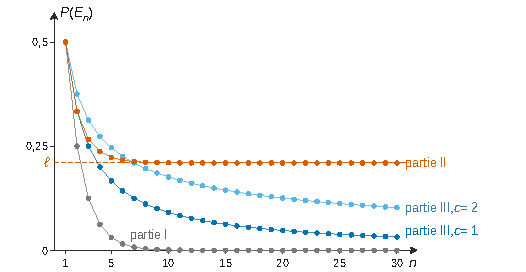
\includegraphics{figures/q12-comparaison-protocoles.pdf}
\caption*{Figure 1 --- P(E\_n) pour n de 1 à 30 dans les trois protocoles : seule
la partie II tend vers une limite ℓ non nulle}
\end{figure}

\begin{center}\rule{0.5\linewidth}{0.5pt}\end{center}

\hypertarget{exercice-2}{%
\section{Exercice 2}\label{exercice-2}}

\hypertarget{partie-i-duxe9composition-en-suxe9rie-de-fourier-calcul-de-sommes-de-suxe9ries-numuxe9riques}{%
\subsection{Partie I --- Décomposition en série de Fourier, calcul de sommes de séries numériques}\label{partie-i-duxe9composition-en-suxe9rie-de-fourier-calcul-de-sommes-de-suxe9ries-numuxe9riques}}

\hypertarget{q13}{%
\subsubsection{Q13}\label{q13}}

Le graphe est celui de \(|x|\) sur \([-\pi,\pi]\), translaté de \(\pm2\pi\) par périodicité : un signal triangulaire continu.

Son minimum \(0\) est atteint en \(-2\pi\), \(0\) et \(2\pi\) ; son maximum \(\pi\) en \(\pm\pi\).

\begin{figure}[H]
\centering
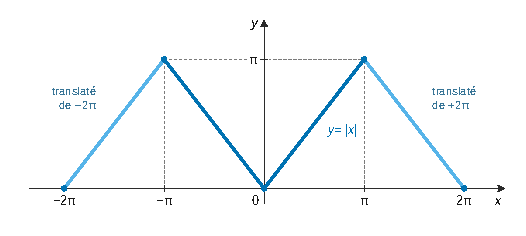
\includegraphics{figures/q13-graphe-signal-triangulaire.pdf}
\caption*{Figure 2 --- Graphe de f sur l'intervalle de −2π à 2π : motif
\textbar x\textbar{} sur l'intervalle de −π à π et ses translatés de ±2π}
\end{figure}

Parité : pour \(x\in\mathbb R\), soit \(k\in\mathbb Z\) tel que \(y=x-2k\pi\in\,]-\pi,\pi]\) ; alors \(-y\in[-\pi,\pi]\) et
\equationajustee{\begin{aligned}
f(-x)&=f(-y)\\
&=|-y|=|y|\\
&=f(y)=f(x).
\end{aligned}}
\textbf{\(f\) est paire.}

Elle n'est pas impaire : sinon \(f(x)=-f(-x)=-f(x)\) donnerait \(f\equiv0\), or \(f(\pi)=\pi\neq0\). \textbf{\(f\) n'est pas impaire.}

\hypertarget{q14.a}{%
\subsubsection{Q14.a)}\label{q14.a}}

Soit \(n\in\mathbb N^*\). La fonction \(x\mapsto|x|\cos(nx)\) est paire et continue, donc par intégration par parties sur le segment \([0,\pi]\) :
\equationajustee{\begin{aligned}
\int_{-\pi}^{\pi}|x|\cos(nx)\,\mathrm dx&=2\int_0^\pi x\cos(nx)\,\mathrm dx\\
&=2\left[\frac{x\sin(nx)}{n}\right]_0^\pi-\frac2n\int_0^\pi\sin(nx)\,\mathrm dx\\
&=\frac{2}{n^2}\big[\cos(nx)\big]_0^\pi ,
\end{aligned}}
\equationajustee{\boxed{\int_{-\pi}^{\pi}|x|\cos(nx)\,\mathrm dx=\frac{2\big((-1)^n-1\big)}{n^2}}.}

\hypertarget{q14.b}{%
\subsubsection{Q14.b)}\label{q14.b}}

\(f\) est continue et \(2\pi\)-périodique. Comme \(f\) est paire, \(x\mapsto f(x)\sin(nx)\) est impaire et \(b_n(f)=\frac1\pi\int_{-\pi}^{\pi}f(x)\sin(nx)\,\mathrm dx=0\) pour tout \(n\ge1\).

Pour \(n\ge1\), d'après Q14.a :
\equationajustee{a_n(f)=\frac1\pi\int_{-\pi}^{\pi}|x|\cos(nx)\,\mathrm dx=\frac{2\big((-1)^n-1\big)}{\pi n^2},}
donc
\equationajustee{\begin{aligned}
a_{2p}&=0\quad(p\ge1),\\
a_{2p+1}&=-\frac{4}{\pi(2p+1)^2}\quad(p\ge0).
\end{aligned}}
Terme constant : au programme de TPC, \(a_0(f)\) est la valeur moyenne de \(f\) sur une période,

\equationajustee{a_0=\frac1{2\pi}\int_{-\pi}^{\pi}|x|\,\mathrm dx=\frac{\pi}{2},}

et la somme partielle s'écrit

\equationajustee{S_n(f)(x)=a_0+\sum_{k=1}^n\big(a_k\cos kx+b_k\sin kx\big).}

Avec l'autre convention (coefficient \(a_0=\frac1\pi\int f\) et terme constant \(\frac{a_0}2\)), on trouverait le même terme constant \(\frac\pi2\).

La série de Fourier de \(f\) est donc, avec \(b_n=0\),
\equationajustee{\boxed{\frac{\pi}{2}-\frac{4}{\pi}\sum_{p\ge0}\frac{\cos\big((2p+1)x\big)}{(2p+1)^2}}.}

\hypertarget{q15}{%
\subsubsection{Q15}\label{q15}}

\(f\) est \(2\pi\)-périodique et continue sur \(\mathbb R\) : \(|x|\) est continue sur \([-\pi,\pi]\) et \(f(-\pi)=f(\pi)=\pi\), ce qui assure le raccord.

Elle est de classe \(\mathcal C^1\) par morceaux : sur \([-\pi,0]\) et \([0,\pi]\) ses restrictions sont affines.

Par le théorème de Dirichlet, la série de Fourier de \(f\) converge en tout point \(x\) vers \(\frac12\big(f(x^+)+f(x^-)\big)\), qui vaut \(f(x)\) par continuité :
\equationajustee{\boxed{\forall x\in\mathbb R,\ f(x)=\frac{\pi}{2}-\frac{4}{\pi}\sum_{p=0}^{+\infty}\frac{\cos\big((2p+1)x\big)}{(2p+1)^2}}.}
En particulier \(|x|=\frac\pi2-\frac4\pi\sum_{p\ge0}\frac{\cos((2p+1)x)}{(2p+1)^2}\) pour \(x\in[-\pi,\pi]\).

\hypertarget{q16.a}{%
\subsubsection{Q16.a)}\label{q16.a}}

En \(x=0\), \(f(0)=0\) et \(\cos 0=1\) : \(0=\frac\pi2-\frac4\pi S\), donc
\equationajustee{\boxed{S=\frac{\pi^2}{8}}.}

\hypertarget{q16.b}{%
\subsubsection{Q16.b)}\label{q16.b}}

Les séries \(R\), \(S\), \(T\) convergent (comparaison à \(\frac1{n^2}\), absolument pour \(T\)). Pour \(N\ge1\), en séparant indices pairs et impairs :
\equationajustee{\begin{aligned}
\sum_{n=1}^{2N}\frac1{n^2}&=\sum_{p=1}^{N}\frac{1}{4p^2}\\
&\quad+\sum_{p=0}^{N-1}\frac{1}{(2p+1)^2}.
\end{aligned}}
En faisant \(N\to+\infty\) (les sommes partielles d'ordre \(2N\) tendent vers \(R\)) :
\equationajustee{\begin{aligned}
R&=\frac R4+S,\\
R&=\frac43S,
\end{aligned}}
\equationajustee{\boxed{R=\frac{\pi^2}{6}}.}

\hypertarget{q16.c}{%
\subsubsection{Q16.c)}\label{q16.c}}

De même, \((-1)^{n-1}\) vaut \(+1\) pour \(n\) impair et \(-1\) pour \(n\) pair :
\equationajustee{\begin{aligned}
\sum_{n=1}^{2N}\frac{(-1)^{n-1}}{n^2}&=\sum_{p=0}^{N-1}\frac1{(2p+1)^2}-\frac14\sum_{p=1}^{N}\frac1{p^2}\\
&\xrightarrow[N\to+\infty]{}S-\frac R4 .
\end{aligned}}
Donc
\equationajustee{\begin{aligned}
T&=S-\frac R4\\
&=\frac{\pi^2}{8}-\frac{\pi^2}{24},
\end{aligned}}
ou encore, puisque \(S=\frac34R\), \(T=\frac R2\) :
\equationajustee{\boxed{T=\frac{\pi^2}{12}}.}

\hypertarget{partie-ii-application-au-calcul-dintuxe9grales}{%
\subsection{Partie II --- Application au calcul d'intégrales}\label{partie-ii-application-au-calcul-dintuxe9grales}}

\hypertarget{q17.a}{%
\subsubsection{Q17.a)}\label{q17.a}}

Soient \(x\ge0\) et \(k\in\mathbb N^*\). Pour \(A>x\), comme \(k>0\),
\equationajustee{\begin{aligned}
\int_x^A\mathrm e^{-kt}\,\mathrm dt&=\frac{\mathrm e^{-kx}-\mathrm e^{-kA}}{k}\\
&\xrightarrow[A\to+\infty]{}\frac{\mathrm e^{-kx}}{k}.
\end{aligned}}
Donc l'intégrale converge et
\equationajustee{\boxed{\int_x^{+\infty}\mathrm e^{-kt}\,\mathrm dt=\frac{\mathrm e^{-kx}}{k}}.}

\hypertarget{q17.b}{%
\subsubsection{Q17.b)}\label{q17.b}}

\(t\mapsto\ln(1+\mathrm e^{-t})\) est continue et positive sur \([0,+\infty[\).

Posons \(\varphi(u)=u-\ln(1+u)\) : \(\varphi'(u)=\frac{u}{1+u}\ge0\) et \(\varphi(0)=0\), donc \(\ln(1+u)\le u\) pour \(u\ge0\). D'où
\equationajustee{0\le\ln(1+\mathrm e^{-t})\le\mathrm e^{-t}.}
Comme \(\int_0^{+\infty}\mathrm e^{-t}\,\mathrm dt\) converge (Q17.a), le théorème de comparaison pour les fonctions positives donne : \textbf{\(\int_0^{+\infty}\ln(1+\mathrm e^{-t})\,\mathrm dt\) converge.}

\hypertarget{q18.a}{%
\subsubsection{Q18.a)}\label{q18.a}}

Avec \(q=-\mathrm e^{-t}\in[-1,0[\), \(q\neq1\) :
\equationajustee{\begin{aligned}
\sum_{k=1}^{n}(-1)^k\mathrm e^{-kt}&=\sum_{k=1}^n q^k\\
&=q\,\frac{1-q^n}{1-q}\\
&=\frac{-\mathrm e^{-t}\big(1-(-1)^n\mathrm e^{-nt}\big)}{1+\mathrm e^{-t}}\\
&=\frac{-\mathrm e^{-t}}{1+\mathrm e^{-t}}+(-1)^n\frac{\mathrm e^{-(n+1)t}}{1+\mathrm e^{-t}},
\end{aligned}}
et comme \((-1)^n=-(-1)^{n+1}\) :
\equationajustee{\boxed{\sum_{k=1}^{n}(-1)^k\mathrm e^{-kt}=\frac{-\mathrm e^{-t}}{1+\mathrm e^{-t}}-(-1)^{n+1}\frac{\mathrm e^{-(n+1)t}}{1+\mathrm e^{-t}}}.}

\hypertarget{q18.b}{%
\subsubsection{Q18.b)}\label{q18.b}}

Soit \(x\ge0\). Toutes les fonctions de Q18.a sont continues sur \([x,+\infty[\), et \(\int_x^{+\infty}\mathrm e^{-kt}\,\mathrm dt\) converge (Q17.a). Les majorations
\equationajustee{\begin{aligned}
0\le\frac{\mathrm e^{-t}}{1+\mathrm e^{-t}}&\le\mathrm e^{-t},\\
0\le\frac{\mathrm e^{-(n+1)t}}{1+\mathrm e^{-t}}&\le\mathrm e^{-(n+1)t}
\end{aligned}}
assurent la convergence des deux autres intégrales. Par linéarité, en intégrant Q18.a sur \([x,+\infty[\) :
\equationajustee{\sum_{k=1}^{n}(-1)^k\frac{\mathrm e^{-kx}}{k}=-\int_x^{+\infty}\frac{\mathrm e^{-t}}{1+\mathrm e^{-t}}\,\mathrm dt-(-1)^{n+1}\int_x^{+\infty}\frac{\mathrm e^{-(n+1)t}}{1+\mathrm e^{-t}}\,\mathrm dt .}
Le membre de gauche vaut \(-h_n(x)\).

Une primitive de \(\frac{\mathrm e^{-t}}{1+\mathrm e^{-t}}\) est \(-\ln(1+\mathrm e^{-t})\), qui tend vers \(0\) en \(+\infty\). Donc \(\int_x^{+\infty}\frac{\mathrm e^{-t}}{1+\mathrm e^{-t}}\,\mathrm dt=\ln(1+\mathrm e^{-x})\). En multipliant par \(-1\) :
\equationajustee{\boxed{\forall x\in\mathbb R_+,\ h_n(x)=\ln\left(1+\mathrm e^{-x}\right)+(-1)^{n+1}\int_x^{+\infty}\frac{\mathrm e^{-(n+1)t}}{1+\mathrm e^{-t}}\,\mathrm dt}.}

\hypertarget{q18.c}{%
\subsubsection{Q18.c)}\label{q18.c}}

L'intégrande étant positif, et comme \(1+\mathrm e^{-t}\ge1\),
\equationajustee{\begin{aligned}
\left|\ln(1+\mathrm e^{-x})-h_n(x)\right|&=\int_x^{+\infty}\frac{\mathrm e^{-(n+1)t}}{1+\mathrm e^{-t}}\,\mathrm dt\\
&\le\int_x^{+\infty}\mathrm e^{-(n+1)t}\,\mathrm dt\\
&=\frac{\mathrm e^{-(n+1)x}}{n+1}.
\end{aligned}}
Comme \(x\ge0\), \(\mathrm e^{-(n+1)x}\le\mathrm e^{-nx}\), et \(\frac1{n+1}\le\frac1n\) :
\equationajustee{\boxed{\forall x\in\mathbb R_+,\ \left|\ln(1+\mathrm e^{-x})-h_n(x)\right|\le\frac{\mathrm e^{-nx}}{n}}.}

\hypertarget{q18.d}{%
\subsubsection{Q18.d)}\label{q18.d}}

Par linéarité et Q17.a (avec \(x=0\)), \(\int_0^{+\infty}h_n\) converge et
\equationajustee{\begin{aligned}
\int_0^{+\infty}h_n(x)\,\mathrm dx&=\sum_{k=1}^{n}\frac{(-1)^{k-1}}{k}\cdot\frac1k\\
&=\sum_{k=1}^{n}\frac{(-1)^{k-1}}{k^2}.
\end{aligned}}
La fonction \(\psi_n=\ln(1+\mathrm e^{-x})-h_n\) est continue et \(|\psi_n(x)|\le\frac{\mathrm e^{-nx}}{n}\), d'intégrale convergente sur \([0,+\infty[\). Donc \(\int_0^{+\infty}\psi_n\) converge absolument et, avec Q17.b et la linéarité,
\equationajustee{\begin{aligned}
\left|\int_0^{+\infty}\ln(1+\mathrm e^{-x})\,\mathrm dx-\sum_{k=1}^{n}\frac{(-1)^{k-1}}{k^2}\right|&=\left|\int_0^{+\infty}\psi_n\right|\\
&\le\int_0^{+\infty}\frac{\mathrm e^{-nx}}{n}\,\mathrm dx\\
&=\frac1n\cdot\frac1n ,
\end{aligned}}
\equationajustee{\boxed{\left|\int_0^{+\infty}\ln(1+\mathrm e^{-x})\,\mathrm dx-\sum_{k=1}^{n}\frac{(-1)^{k-1}}{k^2}\right|\le\frac1{n^2}}.}

\hypertarget{q18.e}{%
\subsubsection{Q18.e)}\label{q18.e}}

Quand \(n\to+\infty\), \(\frac1{n^2}\to0\), donc \(\sum_{k=1}^{n}\frac{(-1)^{k-1}}{k^2}\to\int_0^{+\infty}\ln(1+\mathrm e^{-x})\,\mathrm dx\). Or cette somme partielle tend vers \(T=\frac{\pi^2}{12}\) (Q16.c). Par unicité de la limite :
\equationajustee{\boxed{\int_0^{+\infty}\ln\left(1+\mathrm e^{-x}\right)\mathrm dx=\frac{\pi^2}{12}}.}

\hypertarget{q19}{%
\subsubsection{Q19}\label{q19}}

Convergence : \(G(x)=\frac{x\mathrm e^{-x}}{1+\mathrm e^{-x}}\) est continue et positive. De plus \(0\le G(x)\le x\mathrm e^{-x}\) et \(x\mathrm e^{-x}=o(\mathrm e^{-x/2})\). Comme \(\int_0^{+\infty}\mathrm e^{-x/2}\,\mathrm dx\) converge, \(\int_0^{+\infty}G\) converge.

Intégration par parties sur \([0,A]\), \(A>0\), avec \(u(x)=x\) et \(v(x)=-\ln(1+\mathrm e^{-x})\), de classe \(\mathcal C^1\), \(v'(x)=\frac{\mathrm e^{-x}}{1+\mathrm e^{-x}}\) :
\equationajustee{\begin{aligned}
\int_0^A\frac{x\mathrm e^{-x}}{1+\mathrm e^{-x}}\,\mathrm dx&=\Big[-x\ln(1+\mathrm e^{-x})\Big]_0^A+\int_0^A\ln(1+\mathrm e^{-x})\,\mathrm dx\\
&=-A\ln(1+\mathrm e^{-A})+\int_0^A\ln(1+\mathrm e^{-x})\,\mathrm dx .
\end{aligned}}
Or \(0\le A\ln(1+\mathrm e^{-A})\le A\mathrm e^{-A}\to0\), et le dernier terme tend vers \(\frac{\pi^2}{12}\) (Q18.e). En faisant \(A\to+\infty\) :
\equationajustee{\boxed{\int_0^{+\infty}\frac{x\mathrm e^{-x}}{1+\mathrm e^{-x}}\,\mathrm dx=\frac{\pi^2}{12}}.}

\begin{center}\rule{0.5\linewidth}{0.5pt}\end{center}

\hypertarget{exercice-3}{%
\section{Exercice 3}\label{exercice-3}}

\hypertarget{partie-i-uxe9tude-dun-cas-particulier}{%
\subsection{Partie I --- Étude d'un cas particulier}\label{partie-i-uxe9tude-dun-cas-particulier}}

\hypertarget{q20.a}{%
\subsubsection{Q20.a)}\label{q20.a}}

\((x_1,x_2,x_3)\in\ker f\) si et seulement si
\equationajustee{\begin{cases}-x_1+3x_2+x_3=0\\ x_1-x_2=0\\ -4x_1+6x_2+x_3=0\end{cases}}
La deuxième équation donne \(x_2=x_1\), la première \(x_3=-2x_1\). La troisième, qui s'écrit alors \(2x_1+x_3=0\), est vérifiée.

Donc \(\ker f=\mathrm{Vect}\big((1,1,-2)\big)\) et, ce vecteur étant non nul :
\equationajustee{\boxed{\big((1,1,-2)\big)\text{ est une base de }\ker f,\quad\dim\ker f=1}.}

\hypertarget{q20.b}{%
\subsubsection{Q20.b)}\label{q20.b}}

Par la formule du rang, \(\operatorname{rg}f=2\). Or
\equationajustee{A\begin{pmatrix}2\\1\\0\end{pmatrix}=\begin{pmatrix}1\\1\\-2\end{pmatrix}.}
Le vecteur non nul \((1,1,-2)\) est donc dans \(\ker f\cap\operatorname{Im}f\). \textbf{\(\ker f\) et \(\operatorname{Im}f\) ne sont pas supplémentaires dans \(E\)} (on a même \(\ker f\subset\operatorname{Im}f\)).

\hypertarget{q21}{%
\subsubsection{Q21}\label{q21}}

\equationajustee{\chi_A(X)=\det(XI_3-A)=\begin{vmatrix}X+1&-3&-1\\-1&X+1&0\\4&-6&X-1\end{vmatrix}.}
En développant selon la deuxième ligne :
\equationajustee{\begin{aligned}
\chi_A(X)&=\begin{vmatrix}-3&-1\\-6&X-1\end{vmatrix}+(X+1)\begin{vmatrix}X+1&-1\\4&X-1\end{vmatrix}\\
&=-3(X+1)+(X+1)(X^2+3)\\
&=X^2(X+1).
\end{aligned}}
\equationajustee{\boxed{\mathrm{Sp}(A)=\{0,-1\}},\quad 0\text{ double},\ -1\text{ simple}.}
Le sous-espace propre associé à \(0\) est \(\ker f\), de dimension \(1<2\) : \textbf{\(A\) n'est pas diagonalisable.}

\hypertarget{q22.a}{%
\subsubsection{Q22.a)}\label{q22.a}}

\(\dim E=3\), donc \((e'_1,e'_2,e'_3)\) est une base si et seulement si son déterminant dans \(\mathcal B_0\) est non nul :
\equationajustee{\begin{aligned}
\begin{vmatrix}1&2&a\\1&1&0\\-2&0&b\end{vmatrix}&=a\begin{vmatrix}1&1\\-2&0\end{vmatrix}+b\begin{vmatrix}1&2\\1&1\end{vmatrix}\\
&=2a-b .
\end{aligned}}
\equationajustee{\boxed{(e'_1,e'_2,e'_3)\text{ base de }E\iff b\neq2a}.}

\hypertarget{q22.b}{%
\subsubsection{Q22.b)}\label{q22.b}}

\({\mathrm{Mat}}_{\mathcal B'}(f)=T\) équivaut à :
\equationajustee{\begin{aligned}
f(e'_1)&=0,\\
f(e'_2)&=e'_1,\\
f(e'_3)&=e'_1-e'_3.
\end{aligned}}
Les deux premières égalités sont vraies (Q20.a et Q20.b). Pour la troisième, on calcule
\equationajustee{A\begin{pmatrix}a\\0\\b\end{pmatrix}=\begin{pmatrix}-a+b\\a\\-4a+b\end{pmatrix},}
et \(e'_1-e'_3\) a pour coordonnées \((1-a,1,-2-b)\). La condition équivaut donc à
\equationajustee{\begin{cases}b=1\\a=1\\-4a+2b=-2\end{cases}}
système compatible de solution \(a=b=1\), et \(2a-b=1\neq0\) :

\textbf{\(a=1\) et \(b=1\), soit \(e'_3=(1,0,1)\).}

\hypertarget{q22.c}{%
\subsubsection{Q22.c)}\label{q22.c}}

\equationajustee{\boxed{T^2=\begin{pmatrix}0&0&-1\\0&0&0\\0&0&1\end{pmatrix}}}
\equationajustee{\boxed{T^3=\begin{pmatrix}0&0&1\\0&0&0\\0&0&-1\end{pmatrix}=-T^2}}
Par récurrence :
\equationajustee{\begin{aligned}
T^{p+1}&=T^pT\\
&=(-1)^pT^3\\
&=(-1)^{p+1}T^2 .
\end{aligned}}
D'où
\equationajustee{\boxed{\begin{aligned}
T^0&=I_3,\\
T^1&=T,\\
T^p&=(-1)^pT^2=\begin{pmatrix}0&0&(-1)^{p+1}\\0&0&0\\0&0&(-1)^p\end{pmatrix}\quad(p\ge2).
\end{aligned}}}

\hypertarget{q23}{%
\subsubsection{Q23}\label{q23}}

\({\mathrm{Mat}}_{\mathcal B'}(f^2)=T^2\). Pour \(u\) de coordonnées \((\alpha,\beta,\gamma)\) dans \(\mathcal B'\), \(f^2(u)\) a pour coordonnées \((-\gamma,0,\gamma)\). Donc :

\begin{itemize}
\tightlist
\item
  \(\ker f^2=\mathrm{Vect}(e'_1,e'_2)\), de dimension \(2\) ;
\item
  \(\operatorname{Im}f^2=\mathrm{Vect}(w)\) avec \(w=-e'_1+e'_3\), de dimension \(1\).
\end{itemize}

Si \(z=\lambda w\in\ker f^2\), sa troisième coordonnée \(\lambda\) est nulle : \(\ker f^2\cap\operatorname{Im}f^2=\{0_E\}\).

Comme \(2+1=3=\dim E\) :
\equationajustee{\boxed{E=\ker(f^2)\oplus\operatorname{Im}(f^2)}.}
Dans la base canonique : \(\ker f^2=\mathrm{Vect}\big((1,1,-2),(2,1,0)\big)\) et \(\operatorname{Im}f^2=\mathrm{Vect}\big((0,-1,3)\big)\).

\hypertarget{partie-ii-suites-des-noyaux-et-des-images-des-ituxe9ruxe9s-de-f}{%
\subsection{\texorpdfstring{Partie II --- Suites des noyaux et des images des itérés de \(f\)}{Partie II --- Suites des noyaux et des images des itérés de f}}\label{partie-ii-suites-des-noyaux-et-des-images-des-ituxe9ruxe9s-de-f}}

\hypertarget{q24}{%
\subsubsection{Q24}\label{q24}}

\(f\) bijectif est injectif et surjectif : \(\boxed{\ker f=\{0_E\},\ \operatorname{Im}f=E}\). Alors \(\ker f\cap\operatorname{Im}f=\{0_E\}\) et \(\ker f+\operatorname{Im}f=E\) : \textbf{\(p=1\) convient} (\(1\le1\le n\)).

\hypertarget{q25.a}{%
\subsubsection{Q25.a)}\label{q25.a}}

Si \(f^k(u)=0_E\), alors \(f^{k+1}(u)=f\big(f^k(u)\big)=f(0_E)=0_E\) : \(\boxed{u\in\ker(f^{k+1})}\).

\hypertarget{q25.b}{%
\subsubsection{Q25.b)}\label{q25.b}}

Si \(v=f^{k+1}(w)\), alors \(v=f^k\big(f(w)\big)\) : \(\boxed{v\in\operatorname{Im}(f^k)}\).

\hypertarget{q26.a}{%
\subsubsection{Q26.a)}\label{q26.a}}

Formule du rang : \(\dim\ker f+\operatorname{rg}f=n=\dim\ker f^2+\operatorname{rg}f^2\).

Si \(\ker f=\ker f^2\), alors \(\operatorname{rg}f=\operatorname{rg}f^2\) ; avec \(\operatorname{Im}f^2\subset\operatorname{Im}f\) (Q25.b), deux sous-espaces emboîtés de même dimension finie sont égaux : \(\operatorname{Im}f=\operatorname{Im}f^2\).

Si \(\operatorname{Im}f=\operatorname{Im}f^2\), alors \(\dim\ker f=\dim\ker f^2\) et, avec \(\ker f\subset\ker f^2\) (Q25.a), \(\ker f=\ker f^2\).

\textbf{Conclusion : \(\ker f=\ker f^2\iff\operatorname{Im}f=\operatorname{Im}f^2\).}

\hypertarget{q26.b-i}{%
\subsubsection{Q26.b) i)}\label{q26.b-i}}

Supposons \(E=\ker f\oplus\operatorname{Im}f\) et soit \(u\in\ker f^2\). Par définition de la somme \(E=\ker f+\operatorname{Im}f\), il existe \((u_0,u_1)\in\ker f\times\operatorname{Im}f\) tel que \(u=u_0+u_1\).

Alors \(f(u)=f(u_0)+f(u_1)=f(u_1)\). D'une part \(f(u)=f(u_1)\in\operatorname{Im}f\).

D'autre part \(f\big(f(u)\big)=f^2(u)=0_E\), donc \(f(u)\in\ker f\).

Ainsi \(f(u)\in\ker f\cap\operatorname{Im}f=\{0_E\}\) : \(f(u)=0_E\), \textbf{\(u\in\ker f\)}. Donc \(\ker f^2\subset\ker f\) et, avec Q25.a,
\equationajustee{\boxed{\ker f=\ker f^2}.}

\hypertarget{q26.b-ii}{%
\subsubsection{Q26.b) ii)}\label{q26.b-ii}}

Supposons \(\ker f=\ker f^2\). Soit \(y\in\ker f\cap\operatorname{Im}f\) : \(y=f(x)\) et \(f(y)=f^2(x)=0_E\), donc \(x\in\ker f^2=\ker f\) et \(y=f(x)=0_E\).
\equationajustee{\boxed{\ker f\cap\operatorname{Im}f=\{0_E\}}.}
La somme \(\ker f+\operatorname{Im}f\) est donc directe, de dimension \(\dim\ker f+\operatorname{rg}f=n\) (formule du rang) : elle est égale à \(E\). \textbf{\(\ker f=\ker f^2\Rightarrow E=\ker f\oplus\operatorname{Im}f\).}

\hypertarget{q26.b-iii}{%
\subsubsection{Q26.b) iii)}\label{q26.b-iii}}

Les implications de i) et ii) donnent :

\textbf{\(E=\ker f\oplus\operatorname{Im}f\iff\ker f=\ker f^2\).}

(Avec Q26.a, ces deux propriétés équivalent aussi à \(\operatorname{Im}f=\operatorname{Im}f^2\).)

\hypertarget{q27}{%
\subsubsection{Q27}\label{q27}}

D'après Q25.a, \(\ker f^k\subset\ker f^{k+1}\), donc \(a_k\le a_{k+1}\) : \((a_k)\) est croissante.

Comme \(\ker f^k\) est un sous-espace de \(E\), \(a_k\le n\). Croissante et majorée, \textbf{la suite \((a_k)_{k\in\mathbb N}\) converge} (théorème de la limite monotone).

\hypertarget{q28}{%
\subsubsection{Q28}\label{q28}}

Soit \(q\ge p\). En itérant Q25.a, \(\ker f^p\subset\ker f^{p+1}\subset\dots\subset\ker f^q\). De plus \(a_q=a_p\) : les deux sous-espaces sont emboîtés et de même dimension finie, donc égaux. Pour tout \(q\in\mathbb N^*\) tel que \(q\ge p\) :
\equationajustee{\boxed{\ker(f^q)=\ker(f^p)}.}

\hypertarget{q29}{%
\subsubsection{Q29}\label{q29}}

Posons \(g=f^p\), endomorphisme de \(E\). Les questions Q25 et Q26 n'utilisent que la linéarité et la formule du rang : elles valent pour tout endomorphisme de \(E\), donc pour \(g\).

Comme \(2p\ge p\), Q28 donne \(\ker g^2=\ker f^{2p}=\ker f^p=\ker g\). Par Q26.b appliquée à \(g\) :
\equationajustee{\boxed{E=\ker(f^p)\oplus\operatorname{Im}(f^p)}.}

Complément (\(1\le p\le n\)). Choisissons pour \(p\) le plus petit entier \(\ge1\) tel que \(a_q=a_p\) pour tout \(q\ge p\).

Si \(\ker f^k=\ker f^{k+1}\), alors \(\ker f^{k+1}=\ker f^{k+2}\). En effet, pour \(x\in\ker f^{k+2}\), \(f(x)\in\ker f^{k+1}=\ker f^k\), donc \(x\in\ker f^{k+1}\). La suite des noyaux est alors constante à partir de \(k\).

Par minimalité de \(p\), on a donc \(a_0<a_1<\dots<a_p\) (si \(p\ge2\) ; le cas \(p=1\) est immédiat). D'où \(p\le a_p\le n\), puisque \(a_0=0\).

Ainsi \(1\le p\le n\) et l'objectif de la partie II est atteint (le cas bijectif étant réglé en Q24).

\textbf{FIN}

\end{document}
